\section{Additional Stochastic Forecast Visualizations}

In this section we provide additional visualization of the special ENSO events forecast:
\begin{enumerate}
    \item In Figure \ref{fig:full_stochastic_forecast} we present the stochastic forecast visualization for the entire validation period, using the stochastic ensemble at a lead time of 6 months for each time index.
    \item In Figure \ref{fig:1997_dev} through Figure \ref{fig:2011_lanina} we show the forecast of different models for several samples of notable ENSO events. 
\end{enumerate}

\begin{figure}
    \centering
    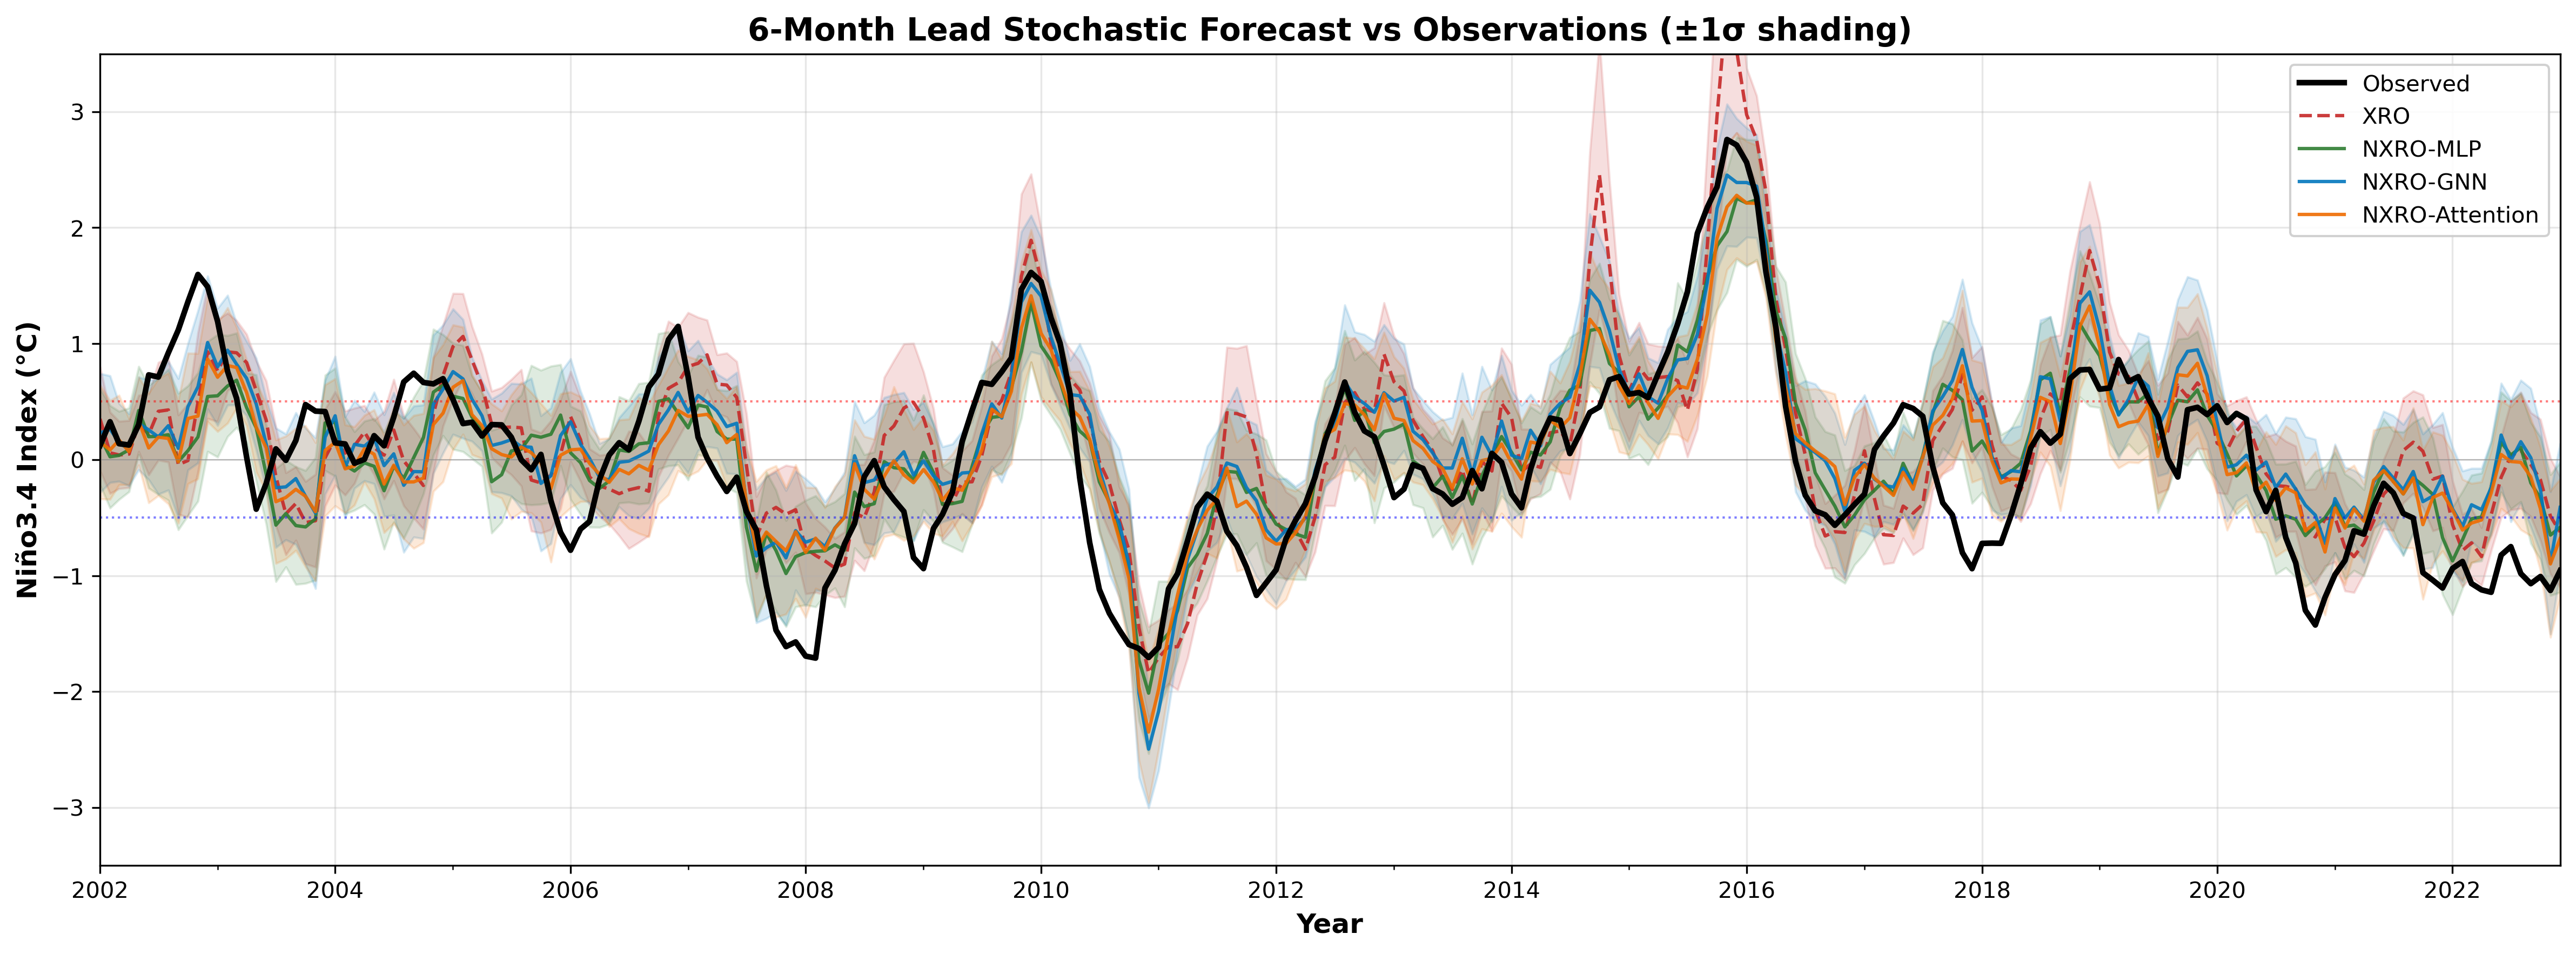
\includegraphics[width=\linewidth]{figures/1h_stochastic_forecast.png}
    \caption{The full stochastic forecast visualization using the ensemble prediction at the validation period. The plot is generated using 6-month forecast at each month.}
    \label{fig:full_stochastic_forecast}
\end{figure}


\begin{figure}[t]
  \centering
  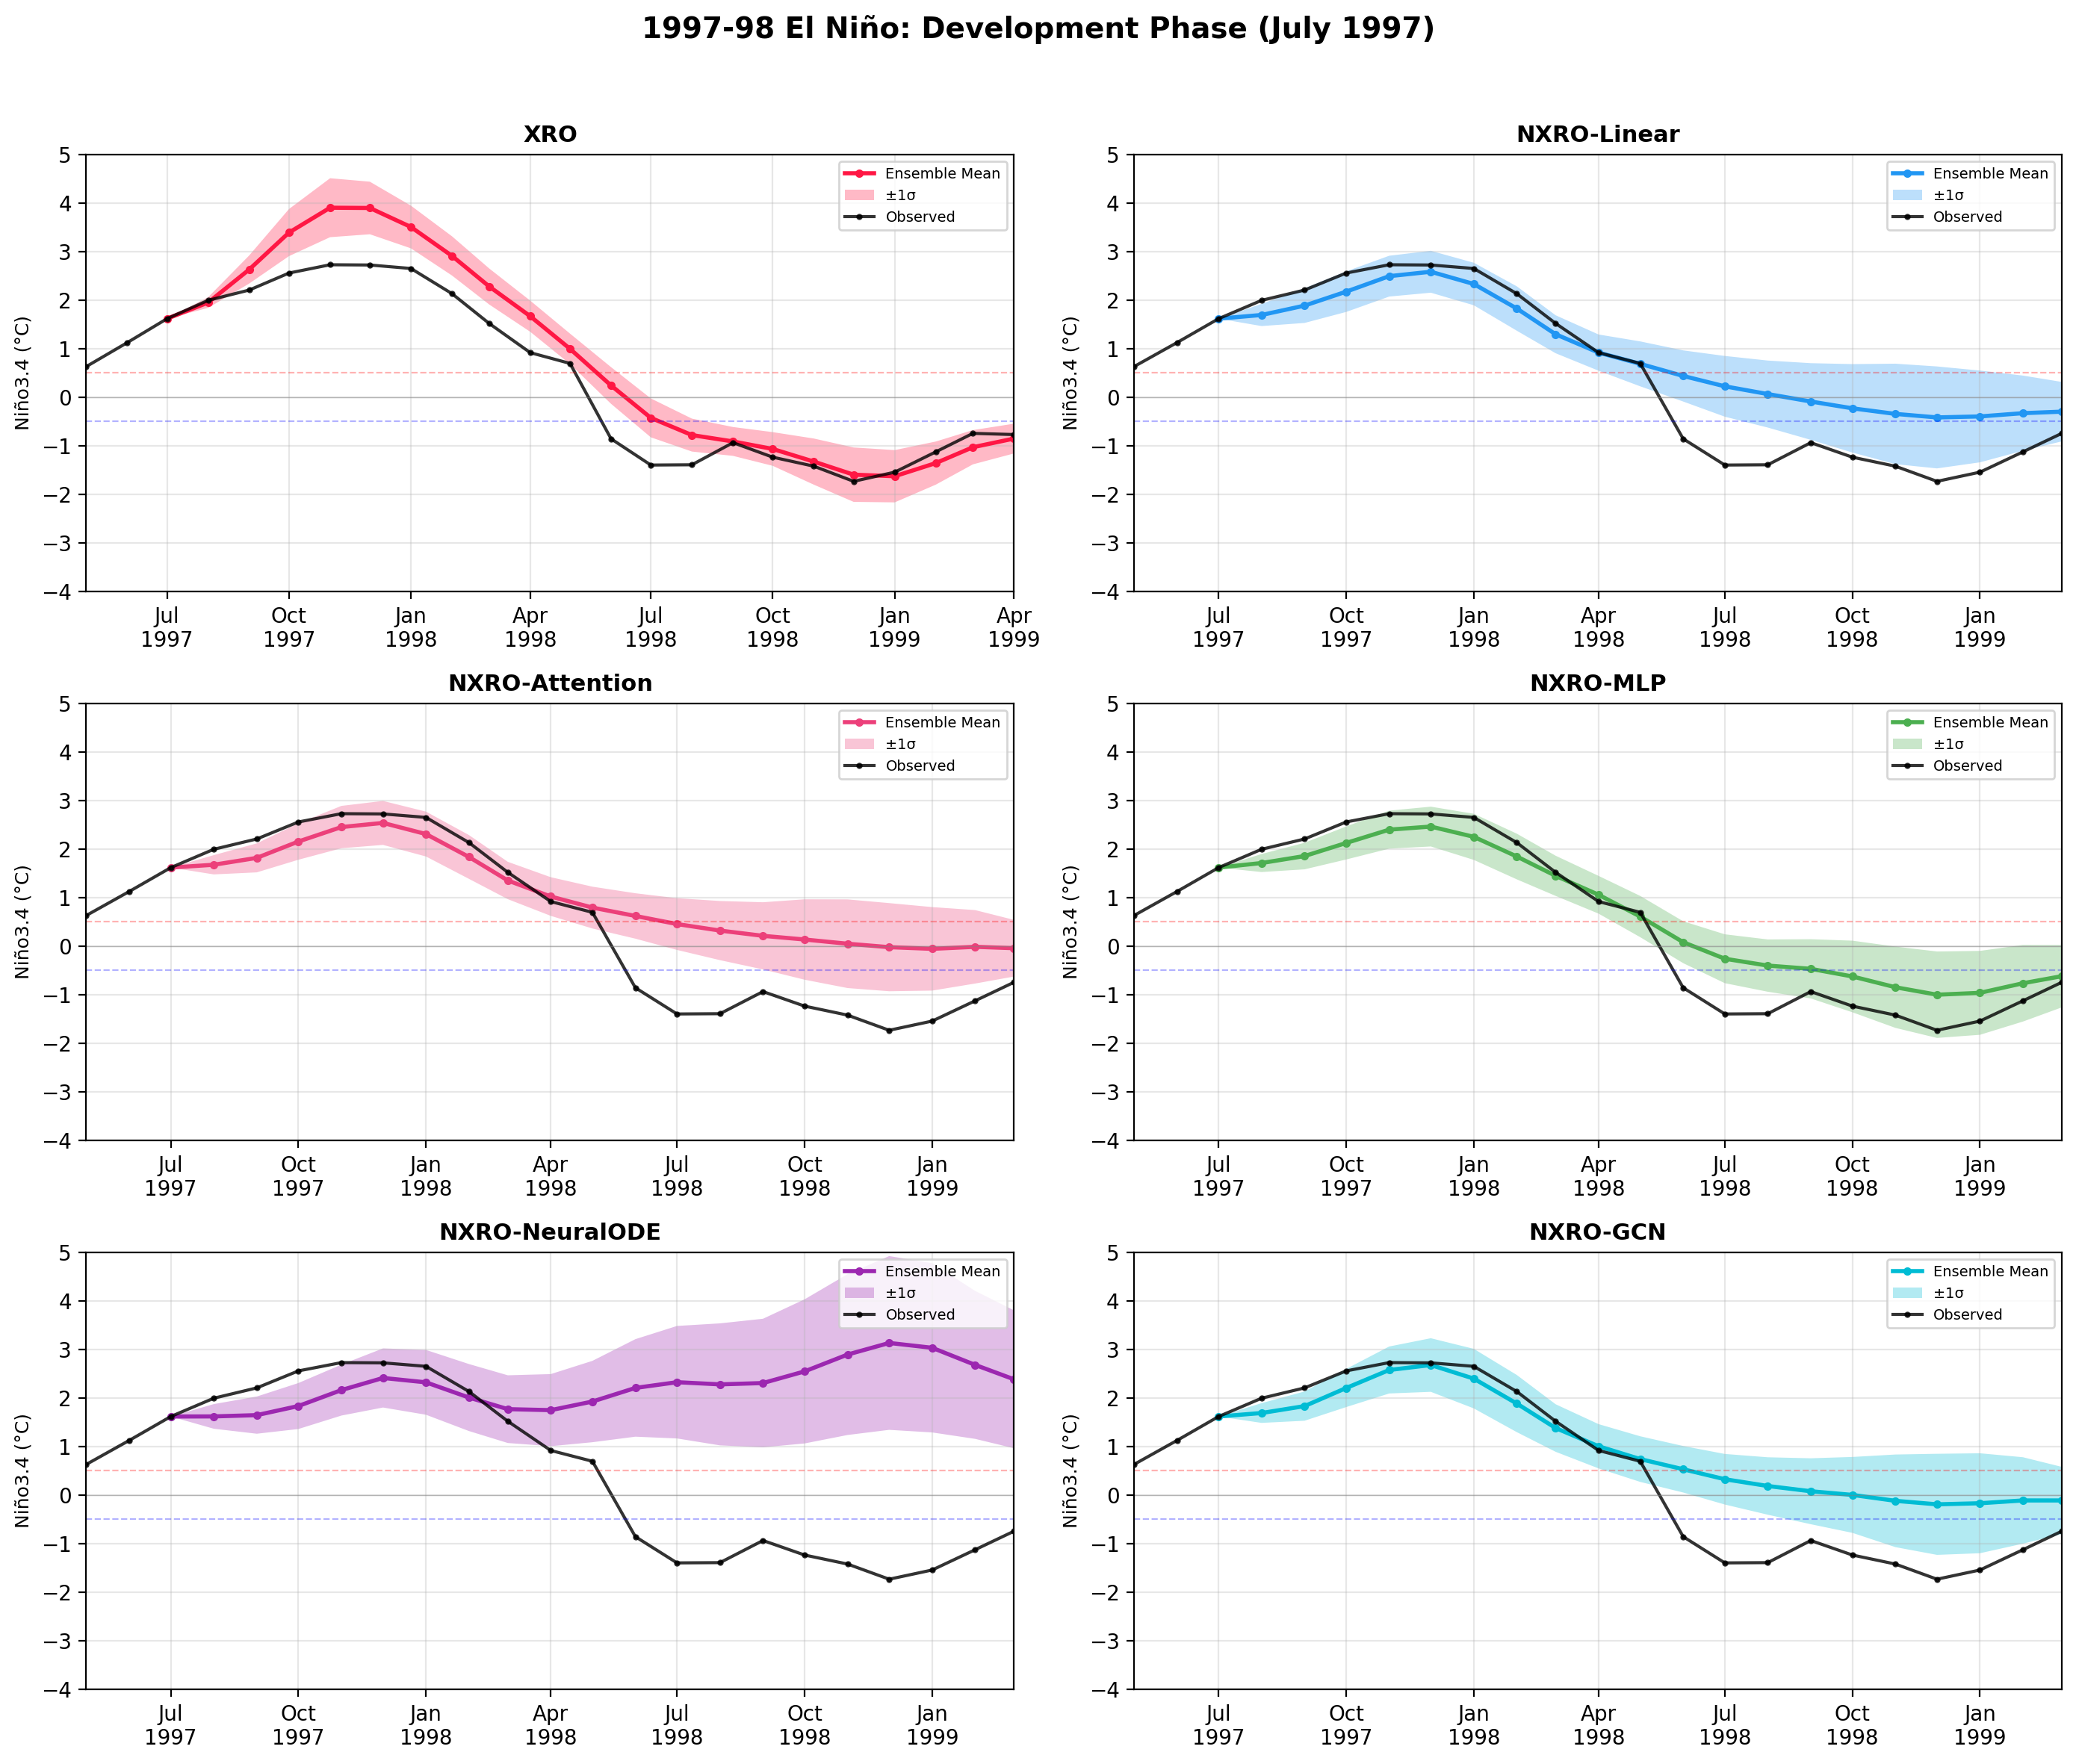
\includegraphics[width=0.8\columnwidth]{figures/elnino_1997_development.png}
  \caption{Stochastic forecast for ENSO development in 1997. Ensemble forecast comparison. Shaded regions show 10--90\% quantile ranges; solid lines show ensemble median; dots show observations.}
  \label{fig:1997_dev}
\end{figure}

\begin{figure}[t]
  \centering
  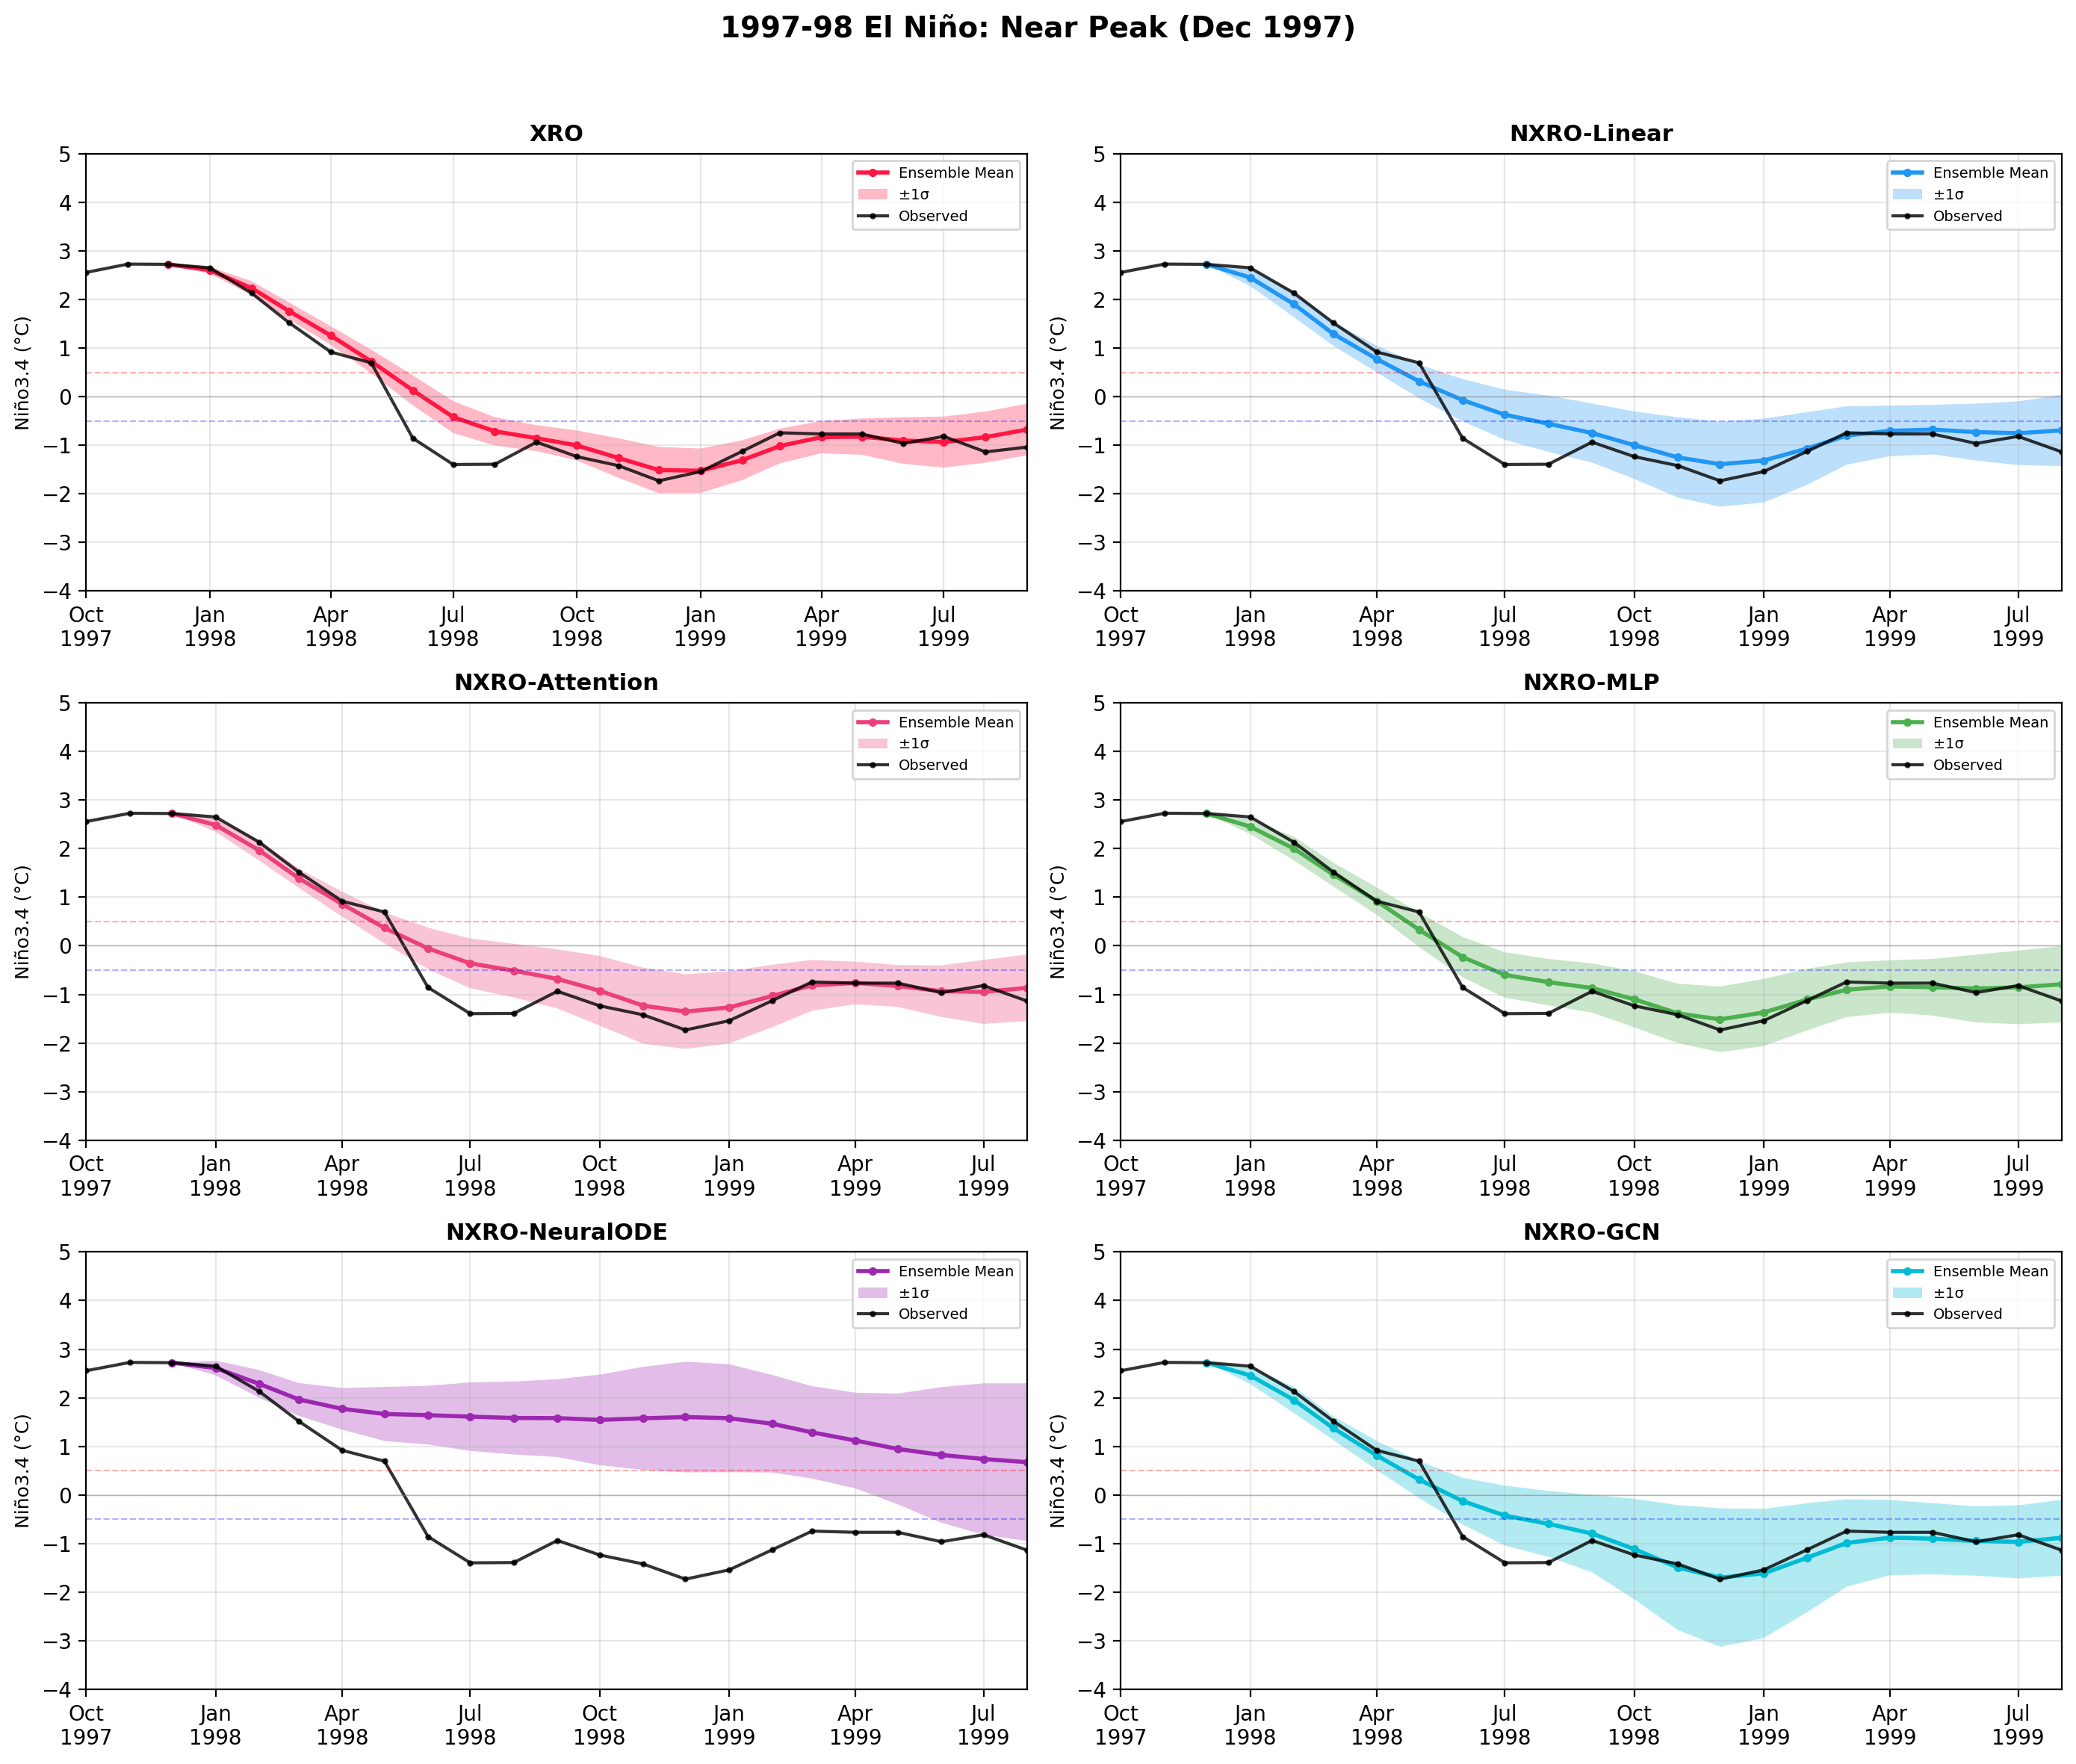
\includegraphics[width=\columnwidth]{figures/elnino_1997_peak.png}
  \caption{Stochastic forecast for ENSO peak in 1997. Ensemble forecast comparison. Shaded regions show 10--90\% quantile ranges; solid lines show ensemble median; dots show observations.}
  \label{fig:1997_peak}
\end{figure}


\begin{figure}[t]
  \centering
  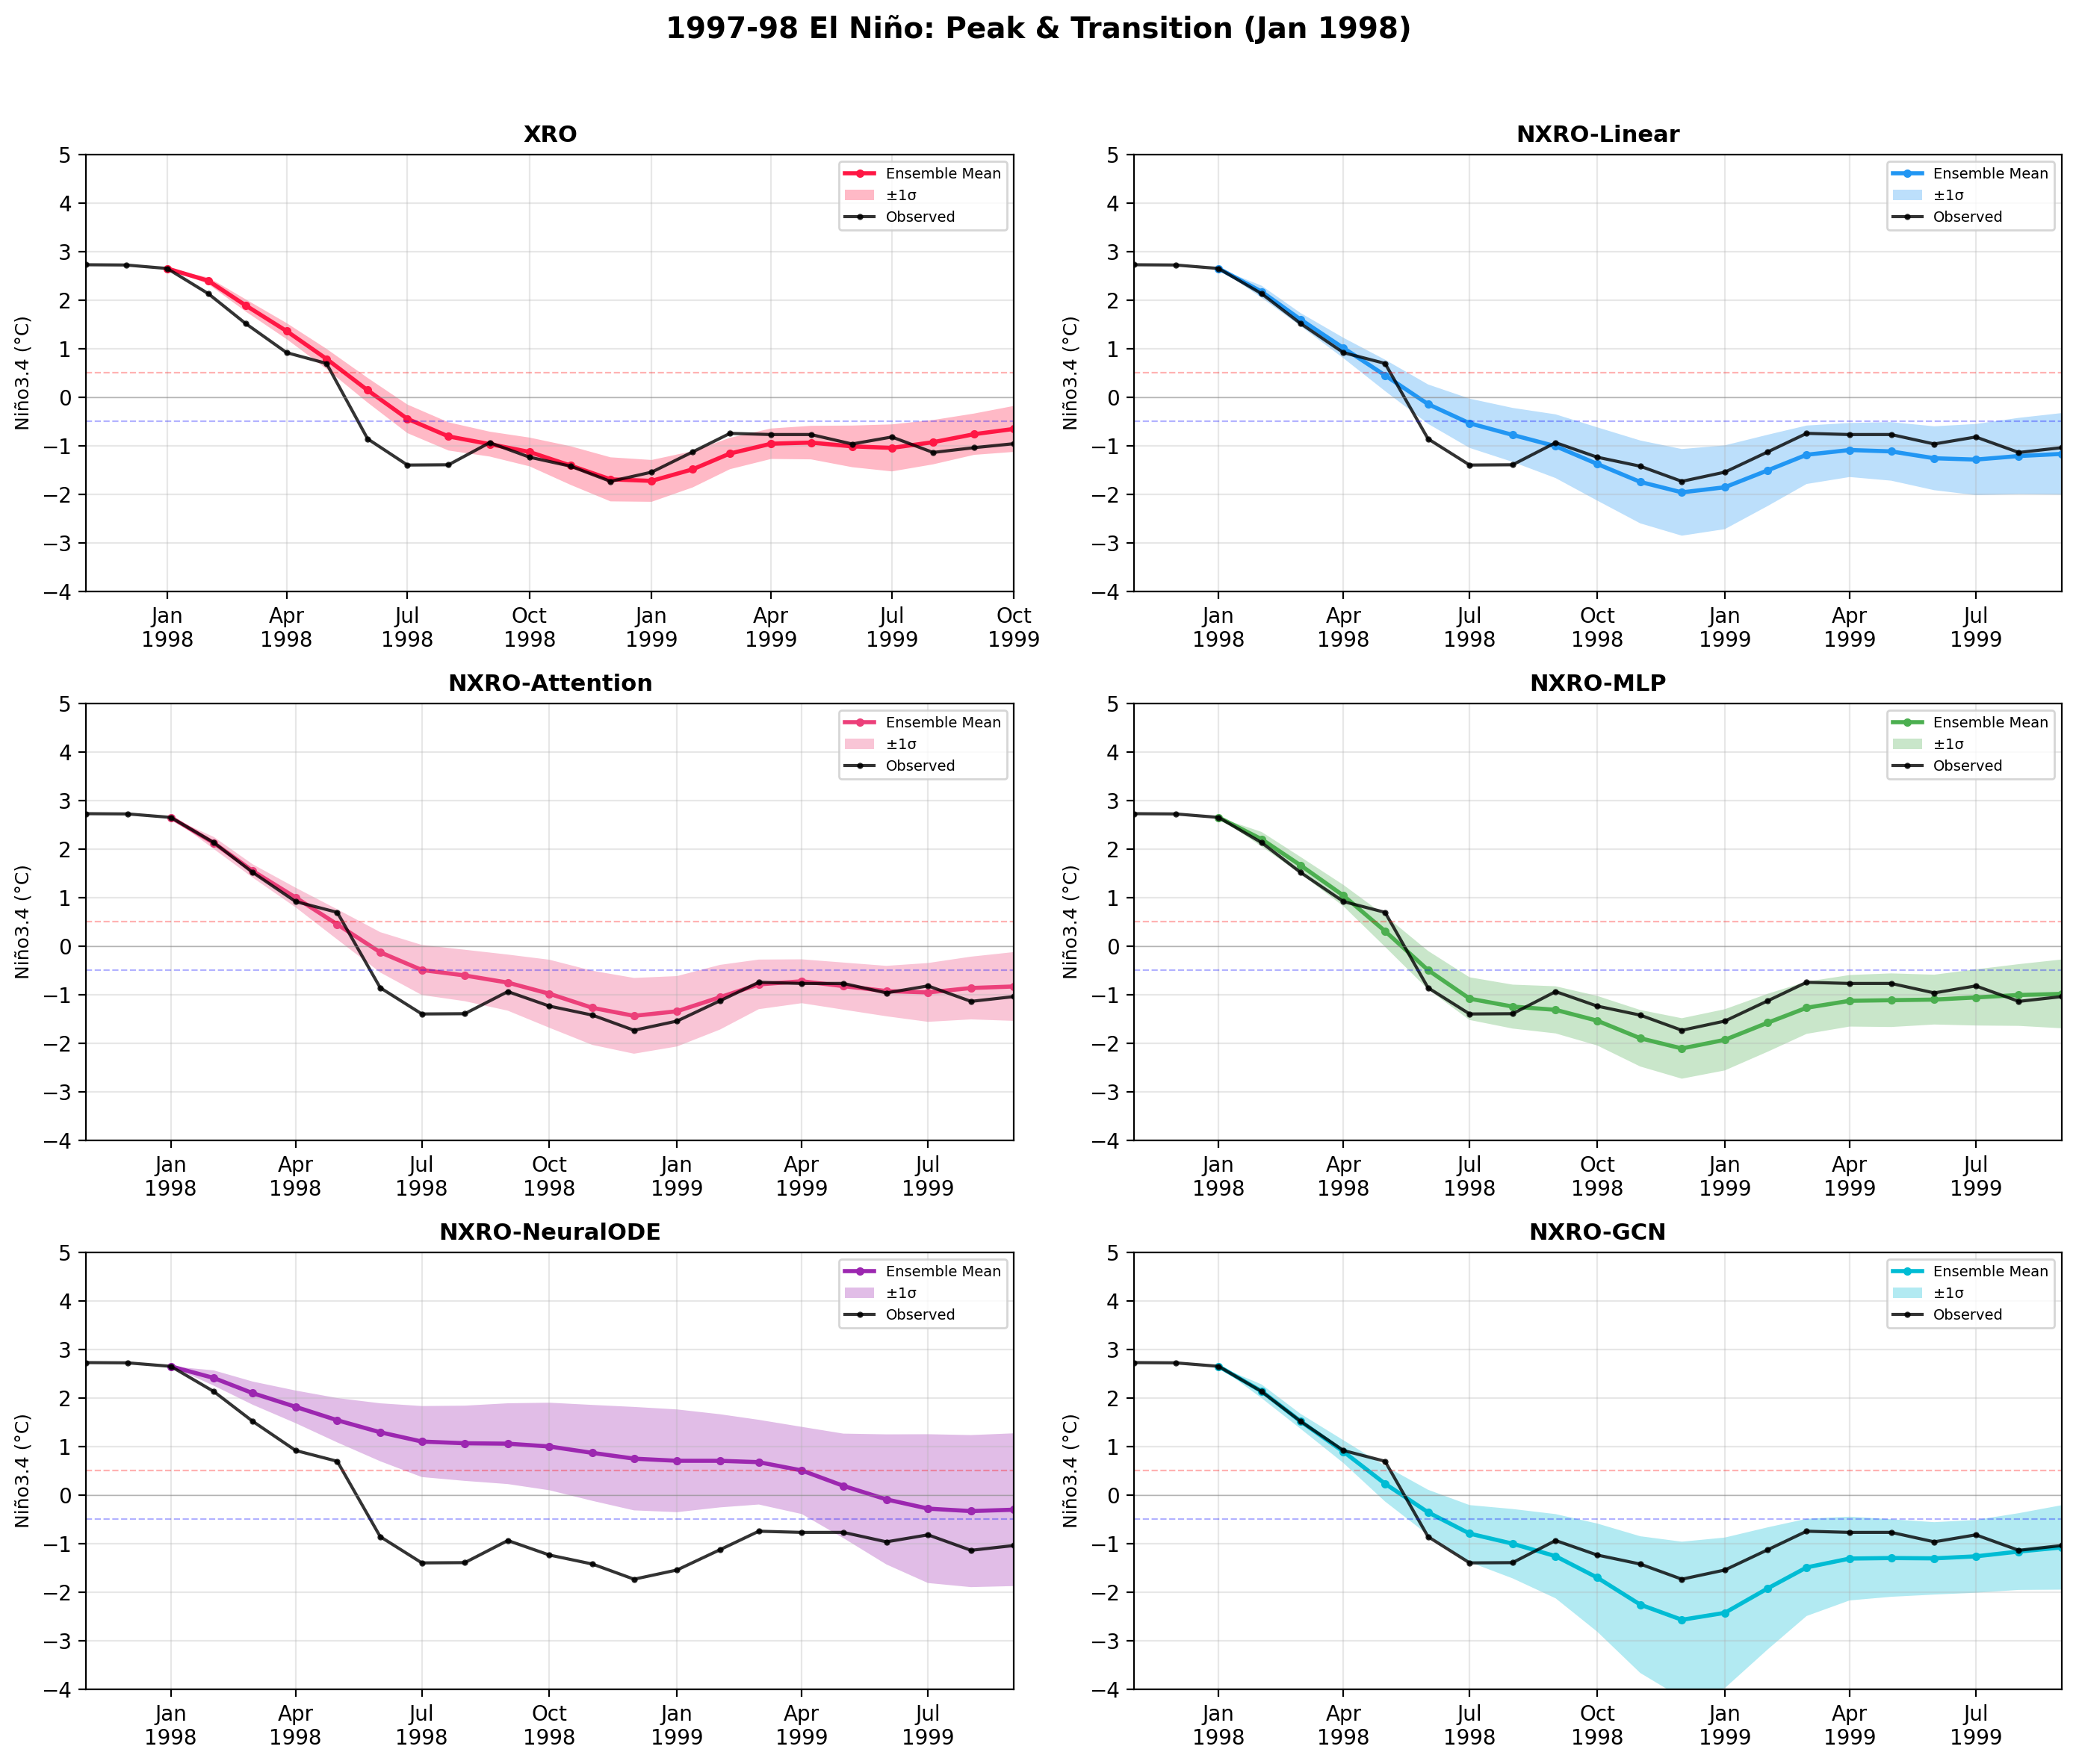
\includegraphics[width=\columnwidth]{figures/elnino_1998_transition.png}
  \caption{Stochastic forecast for ENSO transition in 1998. Ensemble forecast comparison. Shaded regions show 10--90\% quantile ranges; solid lines show ensemble median; dots show observations.}
  \label{fig:1998_trans}
\end{figure}

\begin{figure}[t]
  \centering
  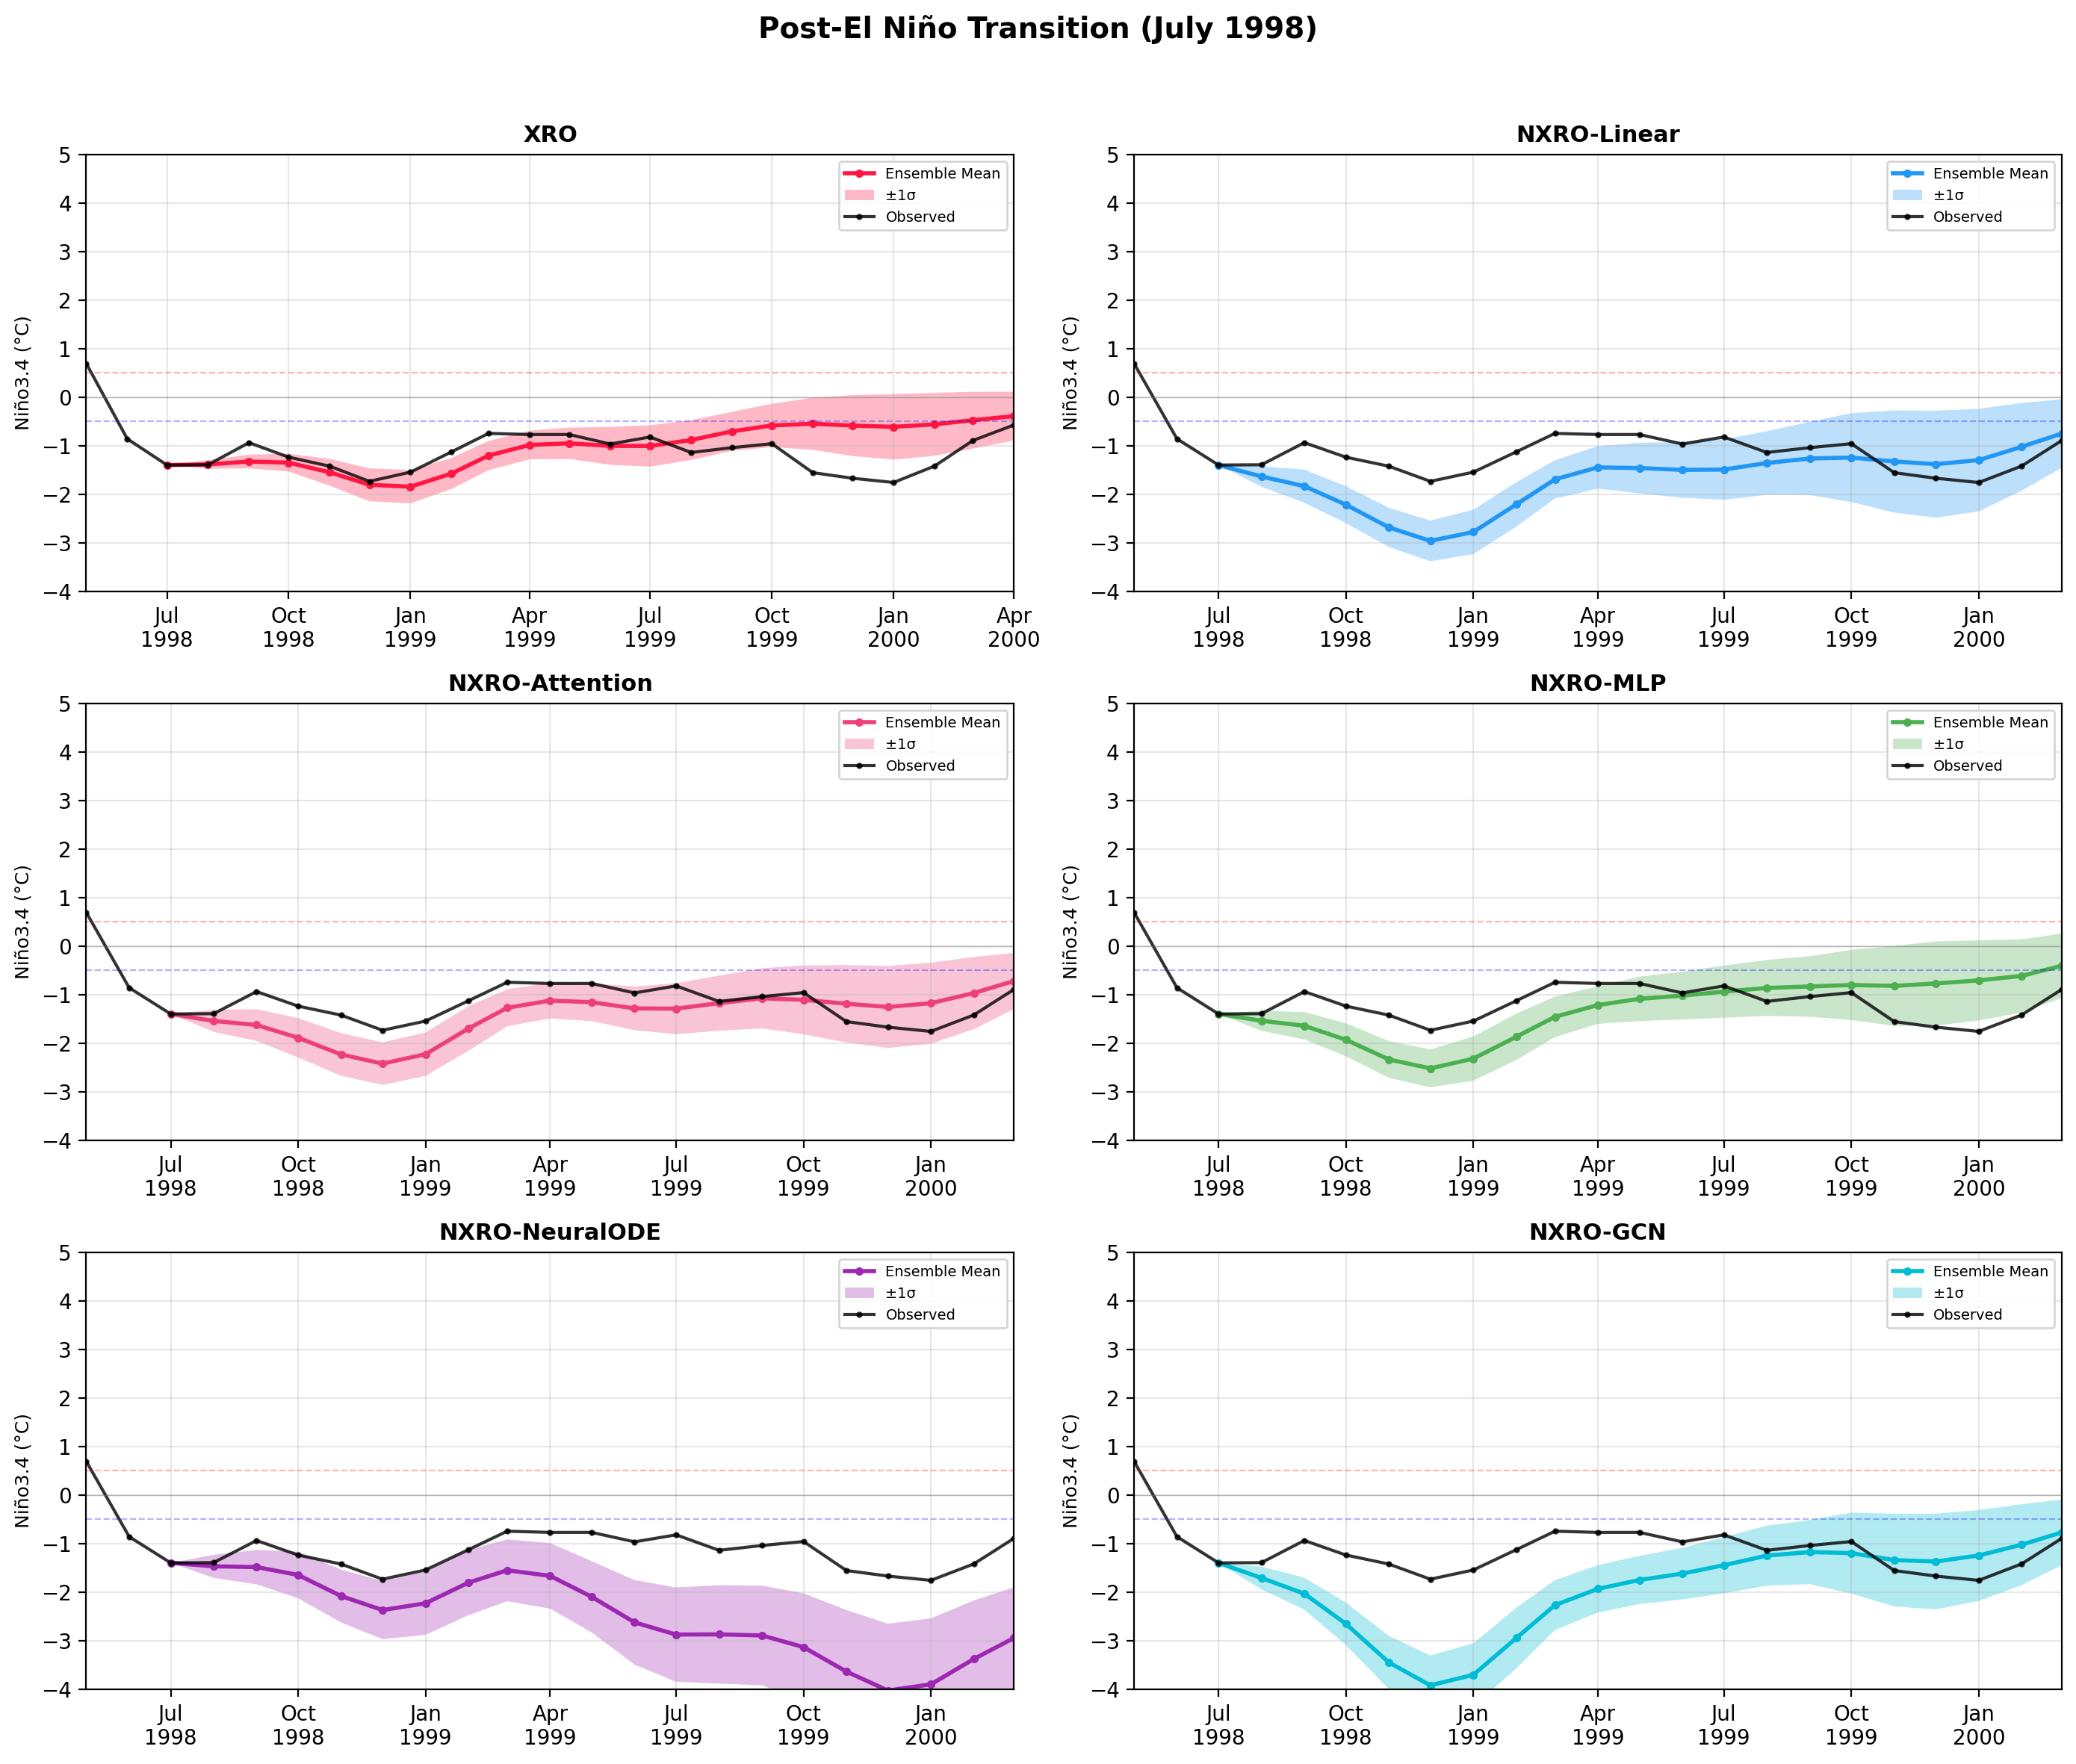
\includegraphics[width=\columnwidth]{figures/transition_1998_summer.png}
  \caption{Stochastic forecast for ENSO summer in 1998. Ensemble forecast comparison. Shaded regions show 10--90\% quantile ranges; solid lines show ensemble median; dots show observations.}
  \label{fig:1998_summer}
\end{figure}

% -------------------- Spring barrier (1997 / 1998) --------------------
\begin{figure}[t]
  \centering
  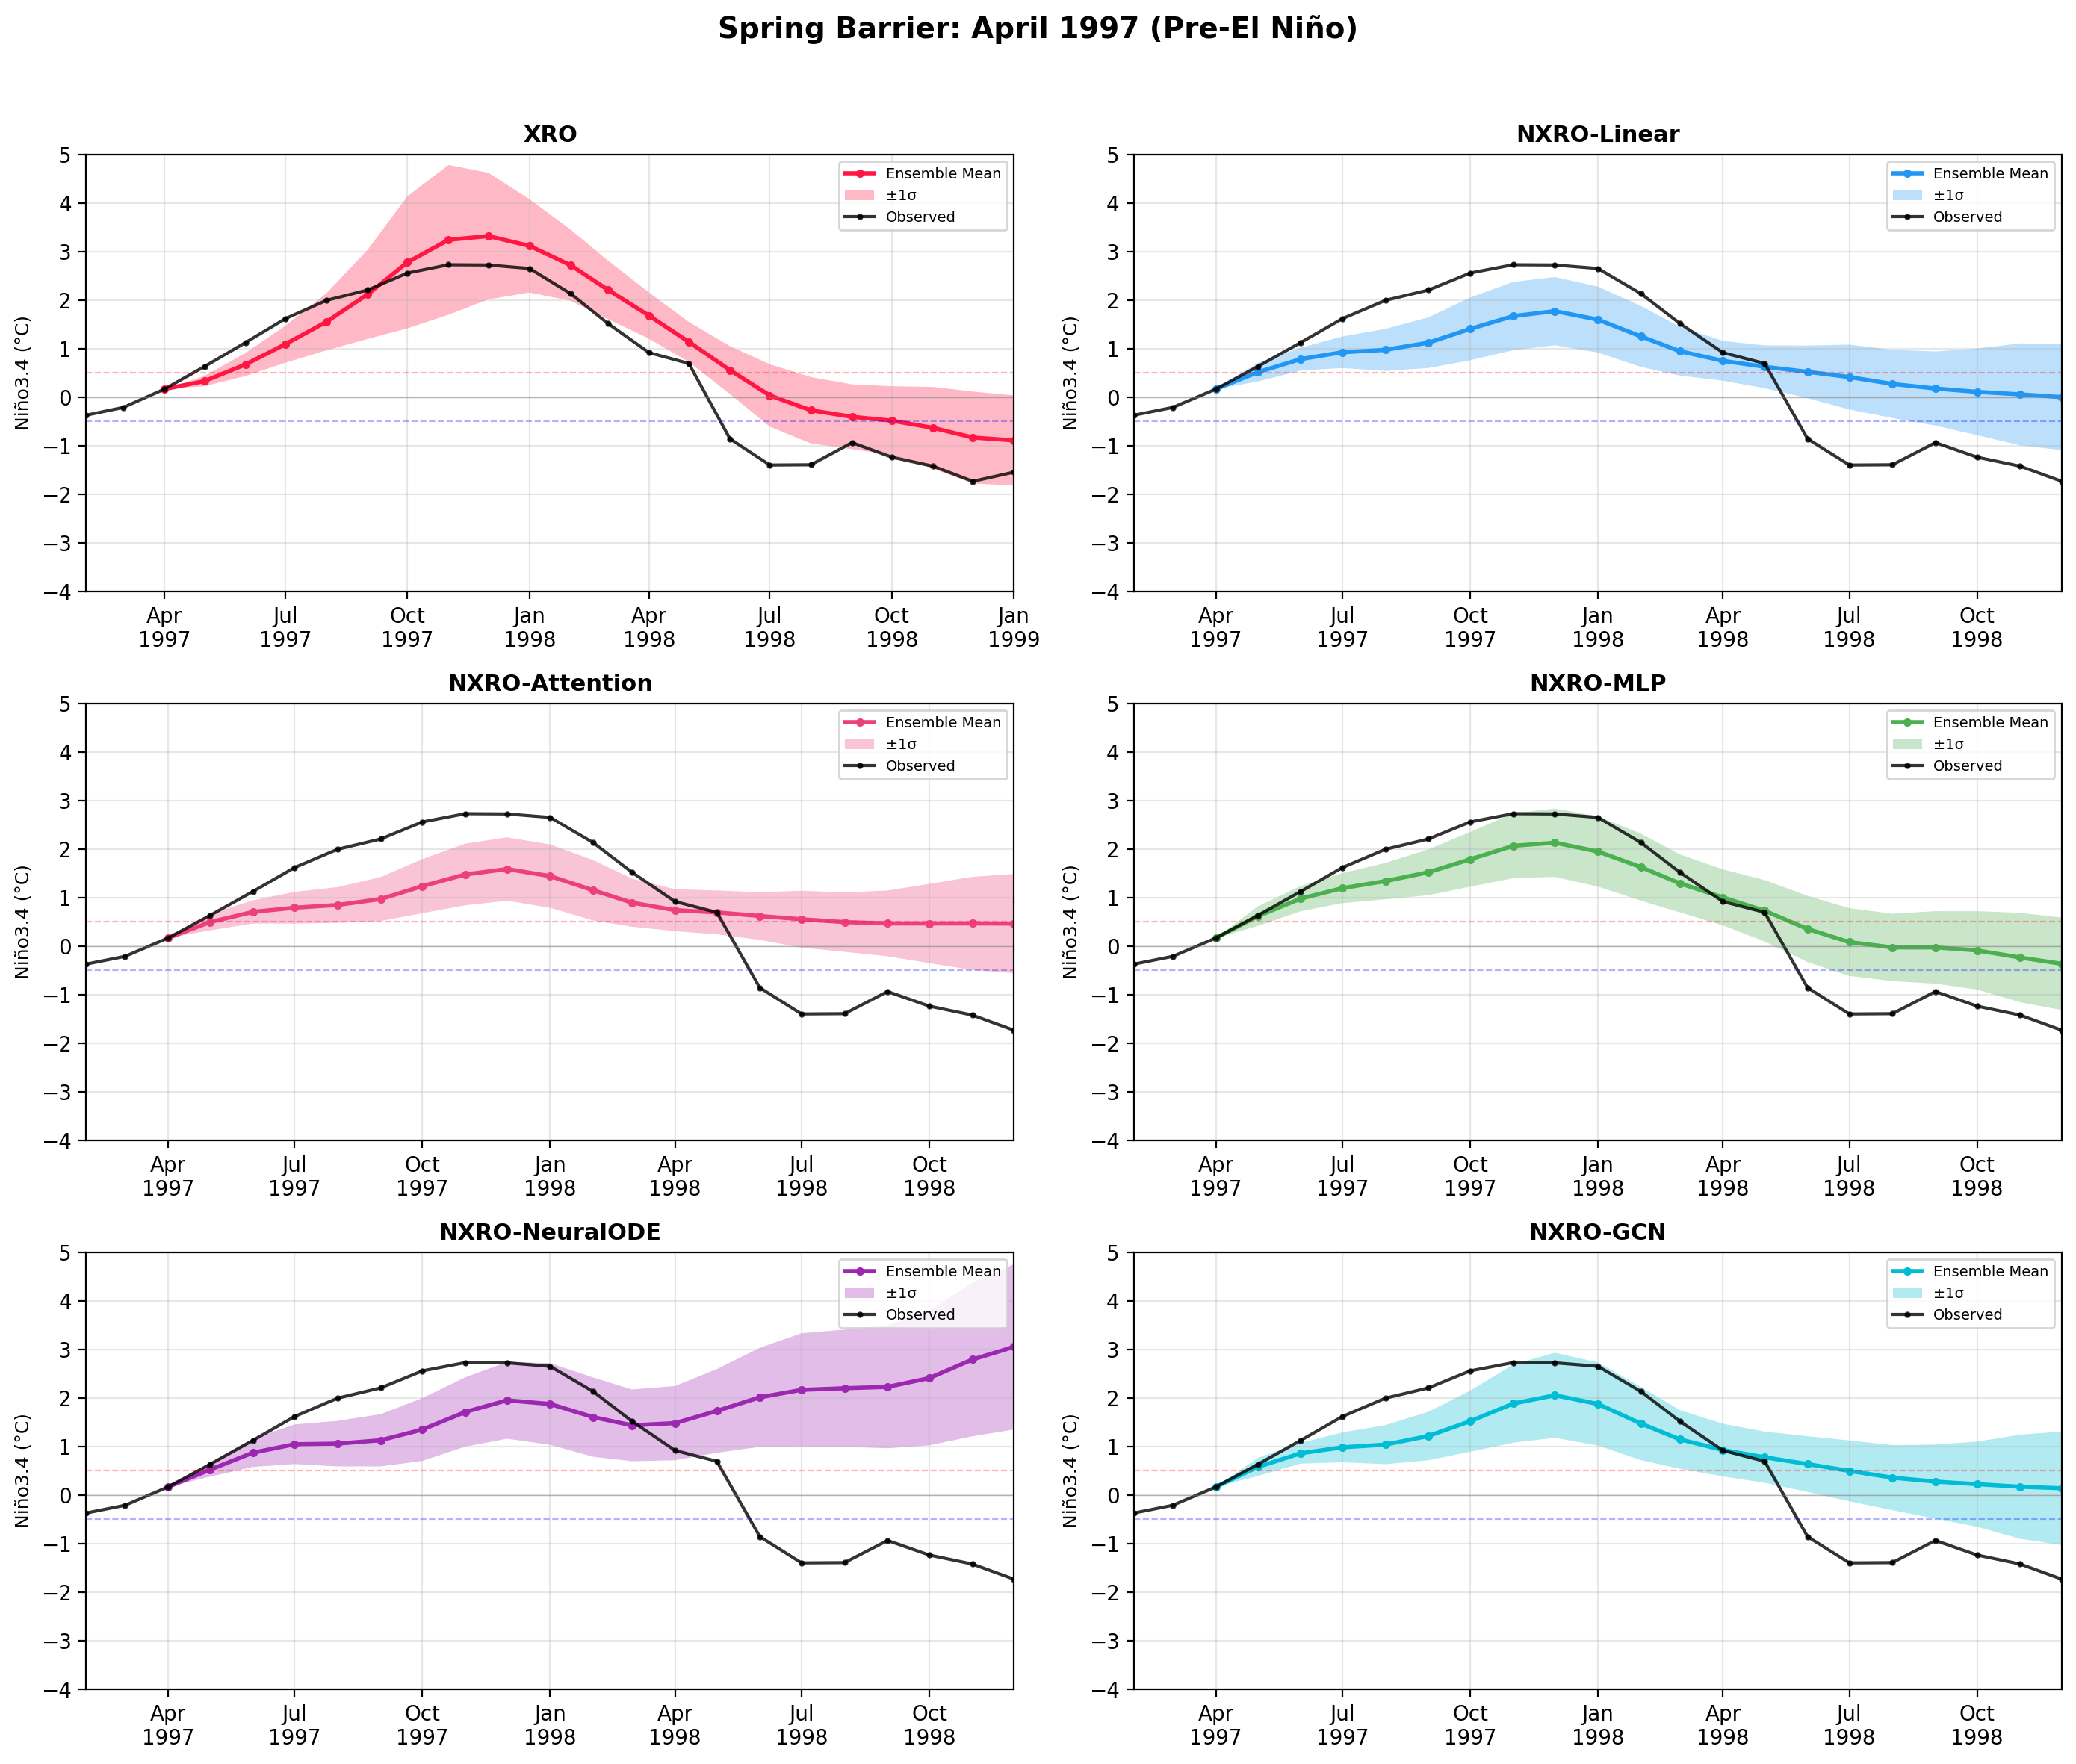
\includegraphics[width=\columnwidth]{figures/spring_barrier_1997.png}
  \caption{Stochastic forecast during spring barrier in 1997. Ensemble forecast comparison. Shaded regions show 10--90\% quantile ranges; solid lines show ensemble median.}
  \label{fig:1997_barrier}
\end{figure}

\begin{figure}[t]
  \centering
  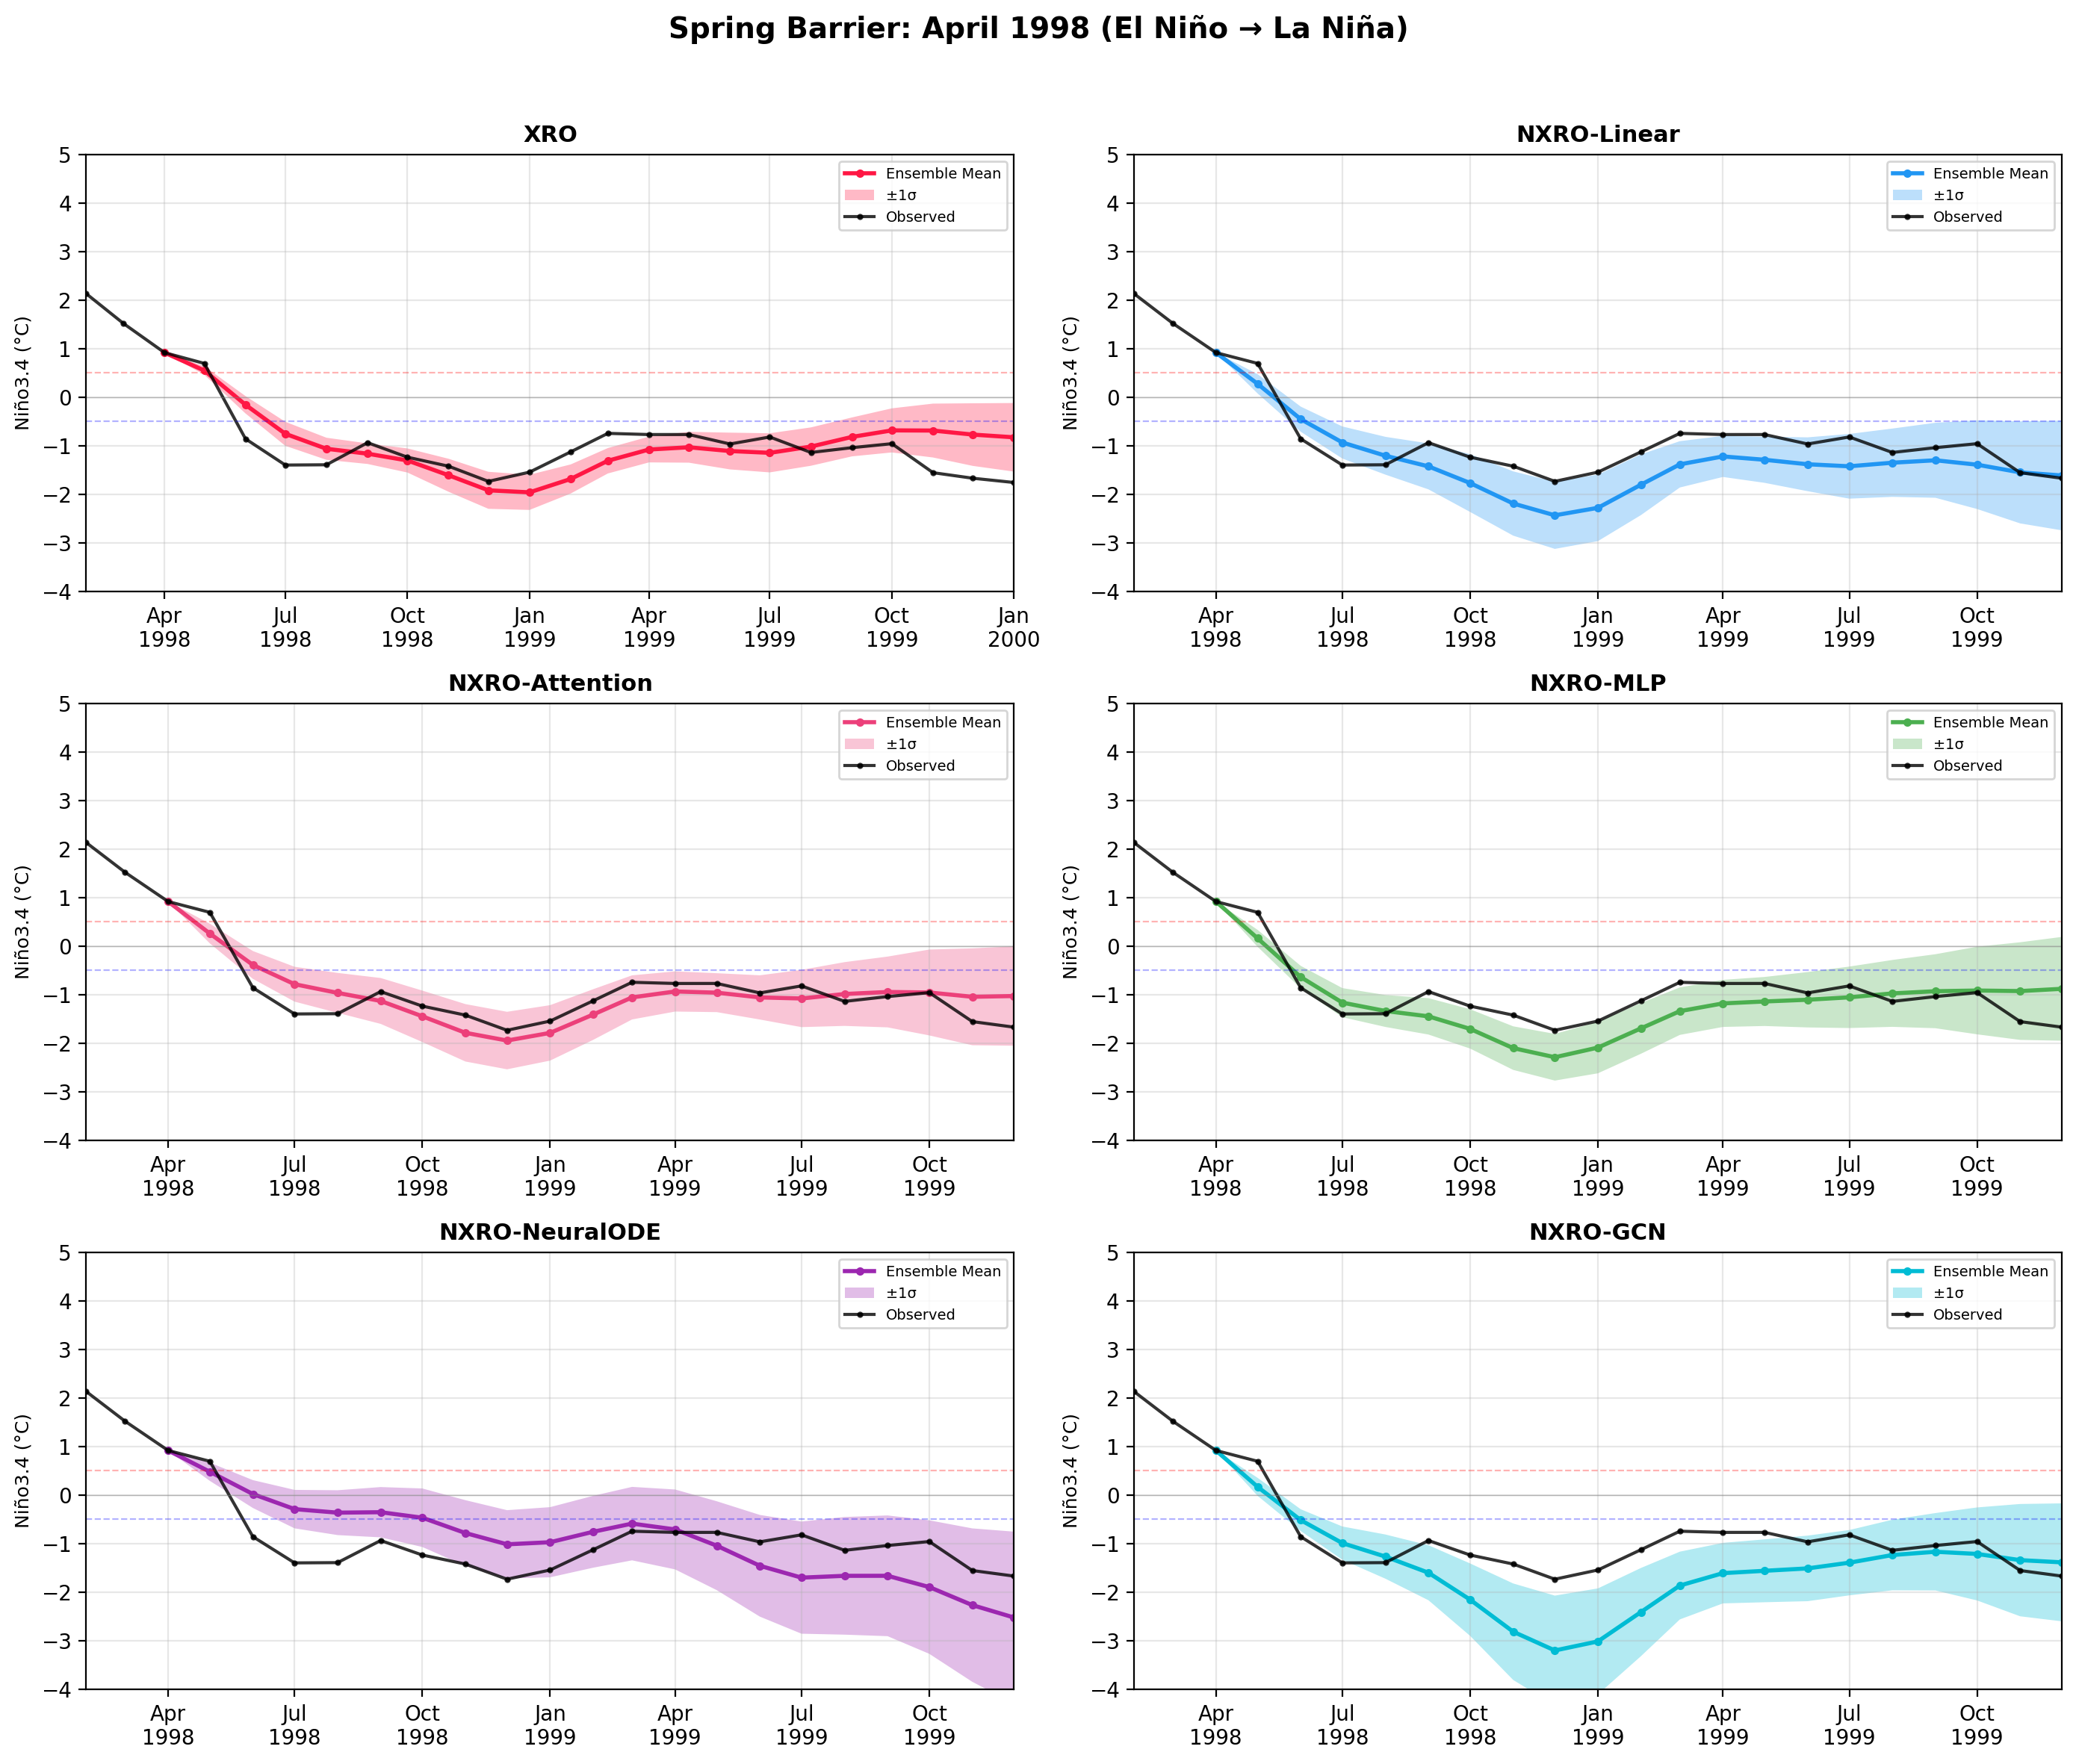
\includegraphics[width=\columnwidth]{figures/spring_barrier_1998.png}
  \caption{Stochastic forecast during spring barrier in 1998. Ensemble forecast comparison. Shaded regions show 10--90\% quantile ranges; solid lines show ensemble median.}
  \label{fig:1998_barrier}
\end{figure}

% -------------------- La Nina (2011 peak / 2010 development) --------------------
\begin{figure}[t]
  \centering
  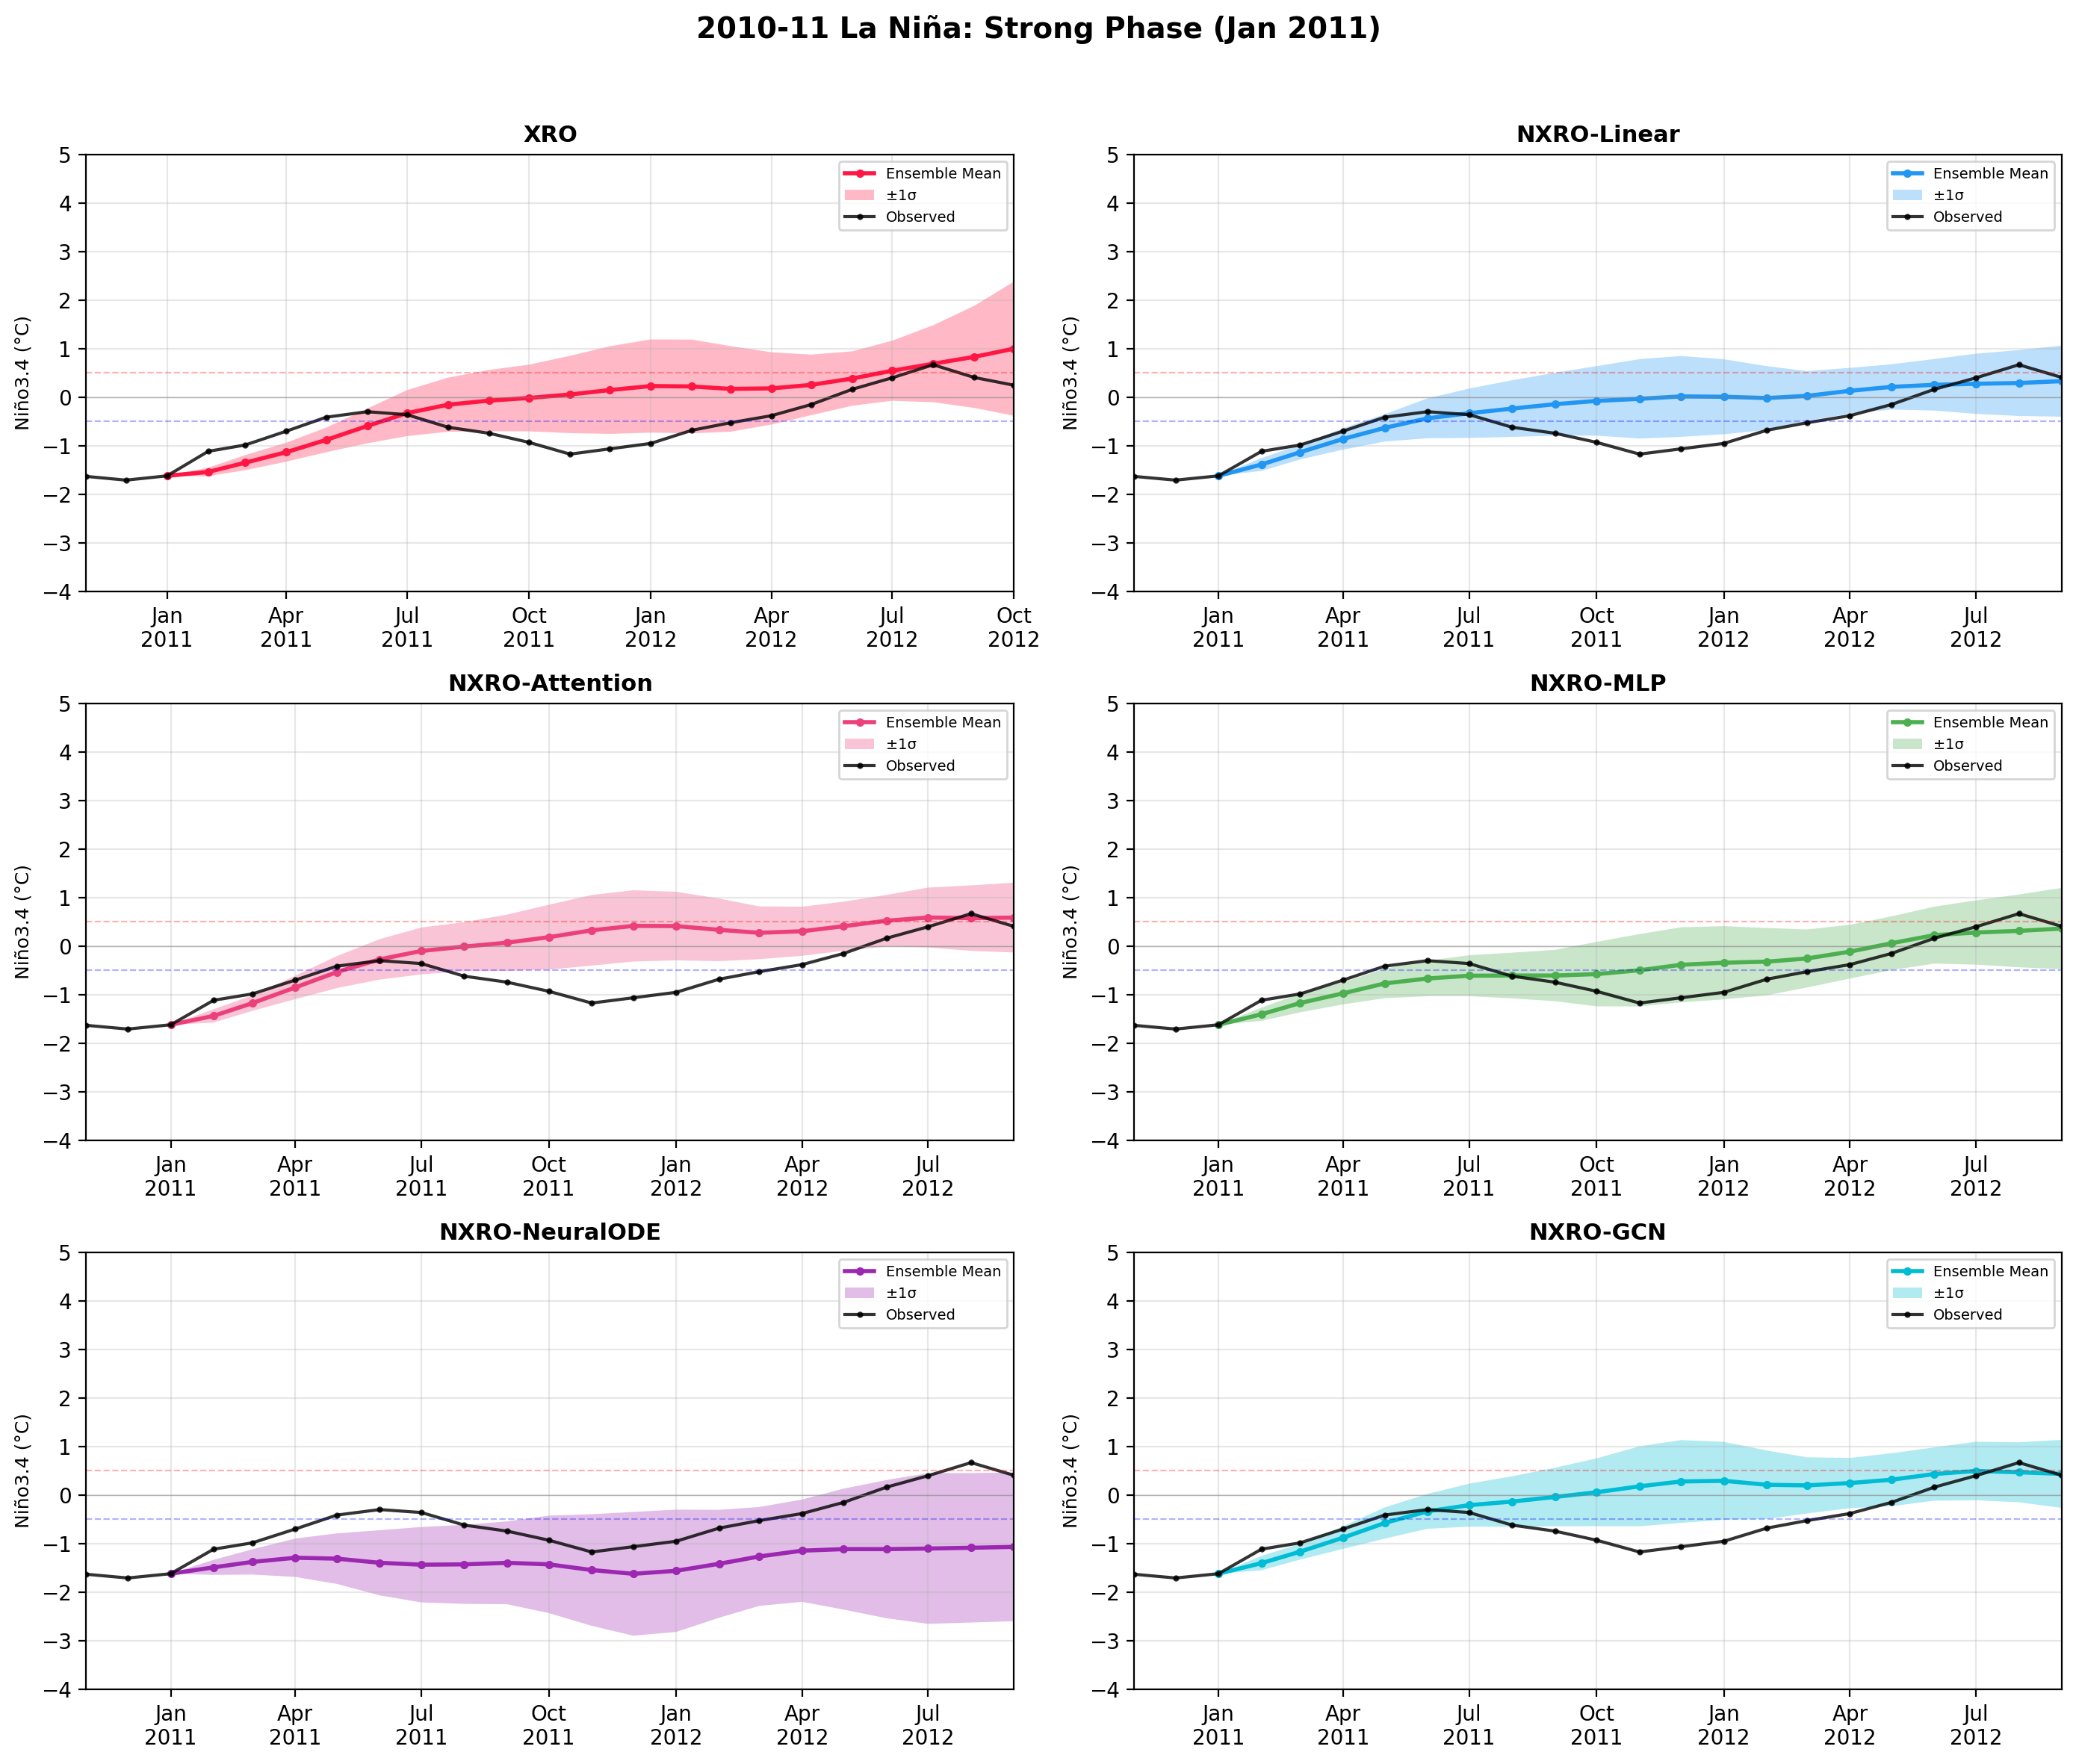
\includegraphics[width=\columnwidth]{figures/lanina_2011_peak.png}
  \caption{Stochastic forecast for the 2011 La Ni\~na peak. Ensemble forecast comparison.}
  \label{fig:2011_lanina}
\end{figure}

\begin{figure}[t]
  \centering
  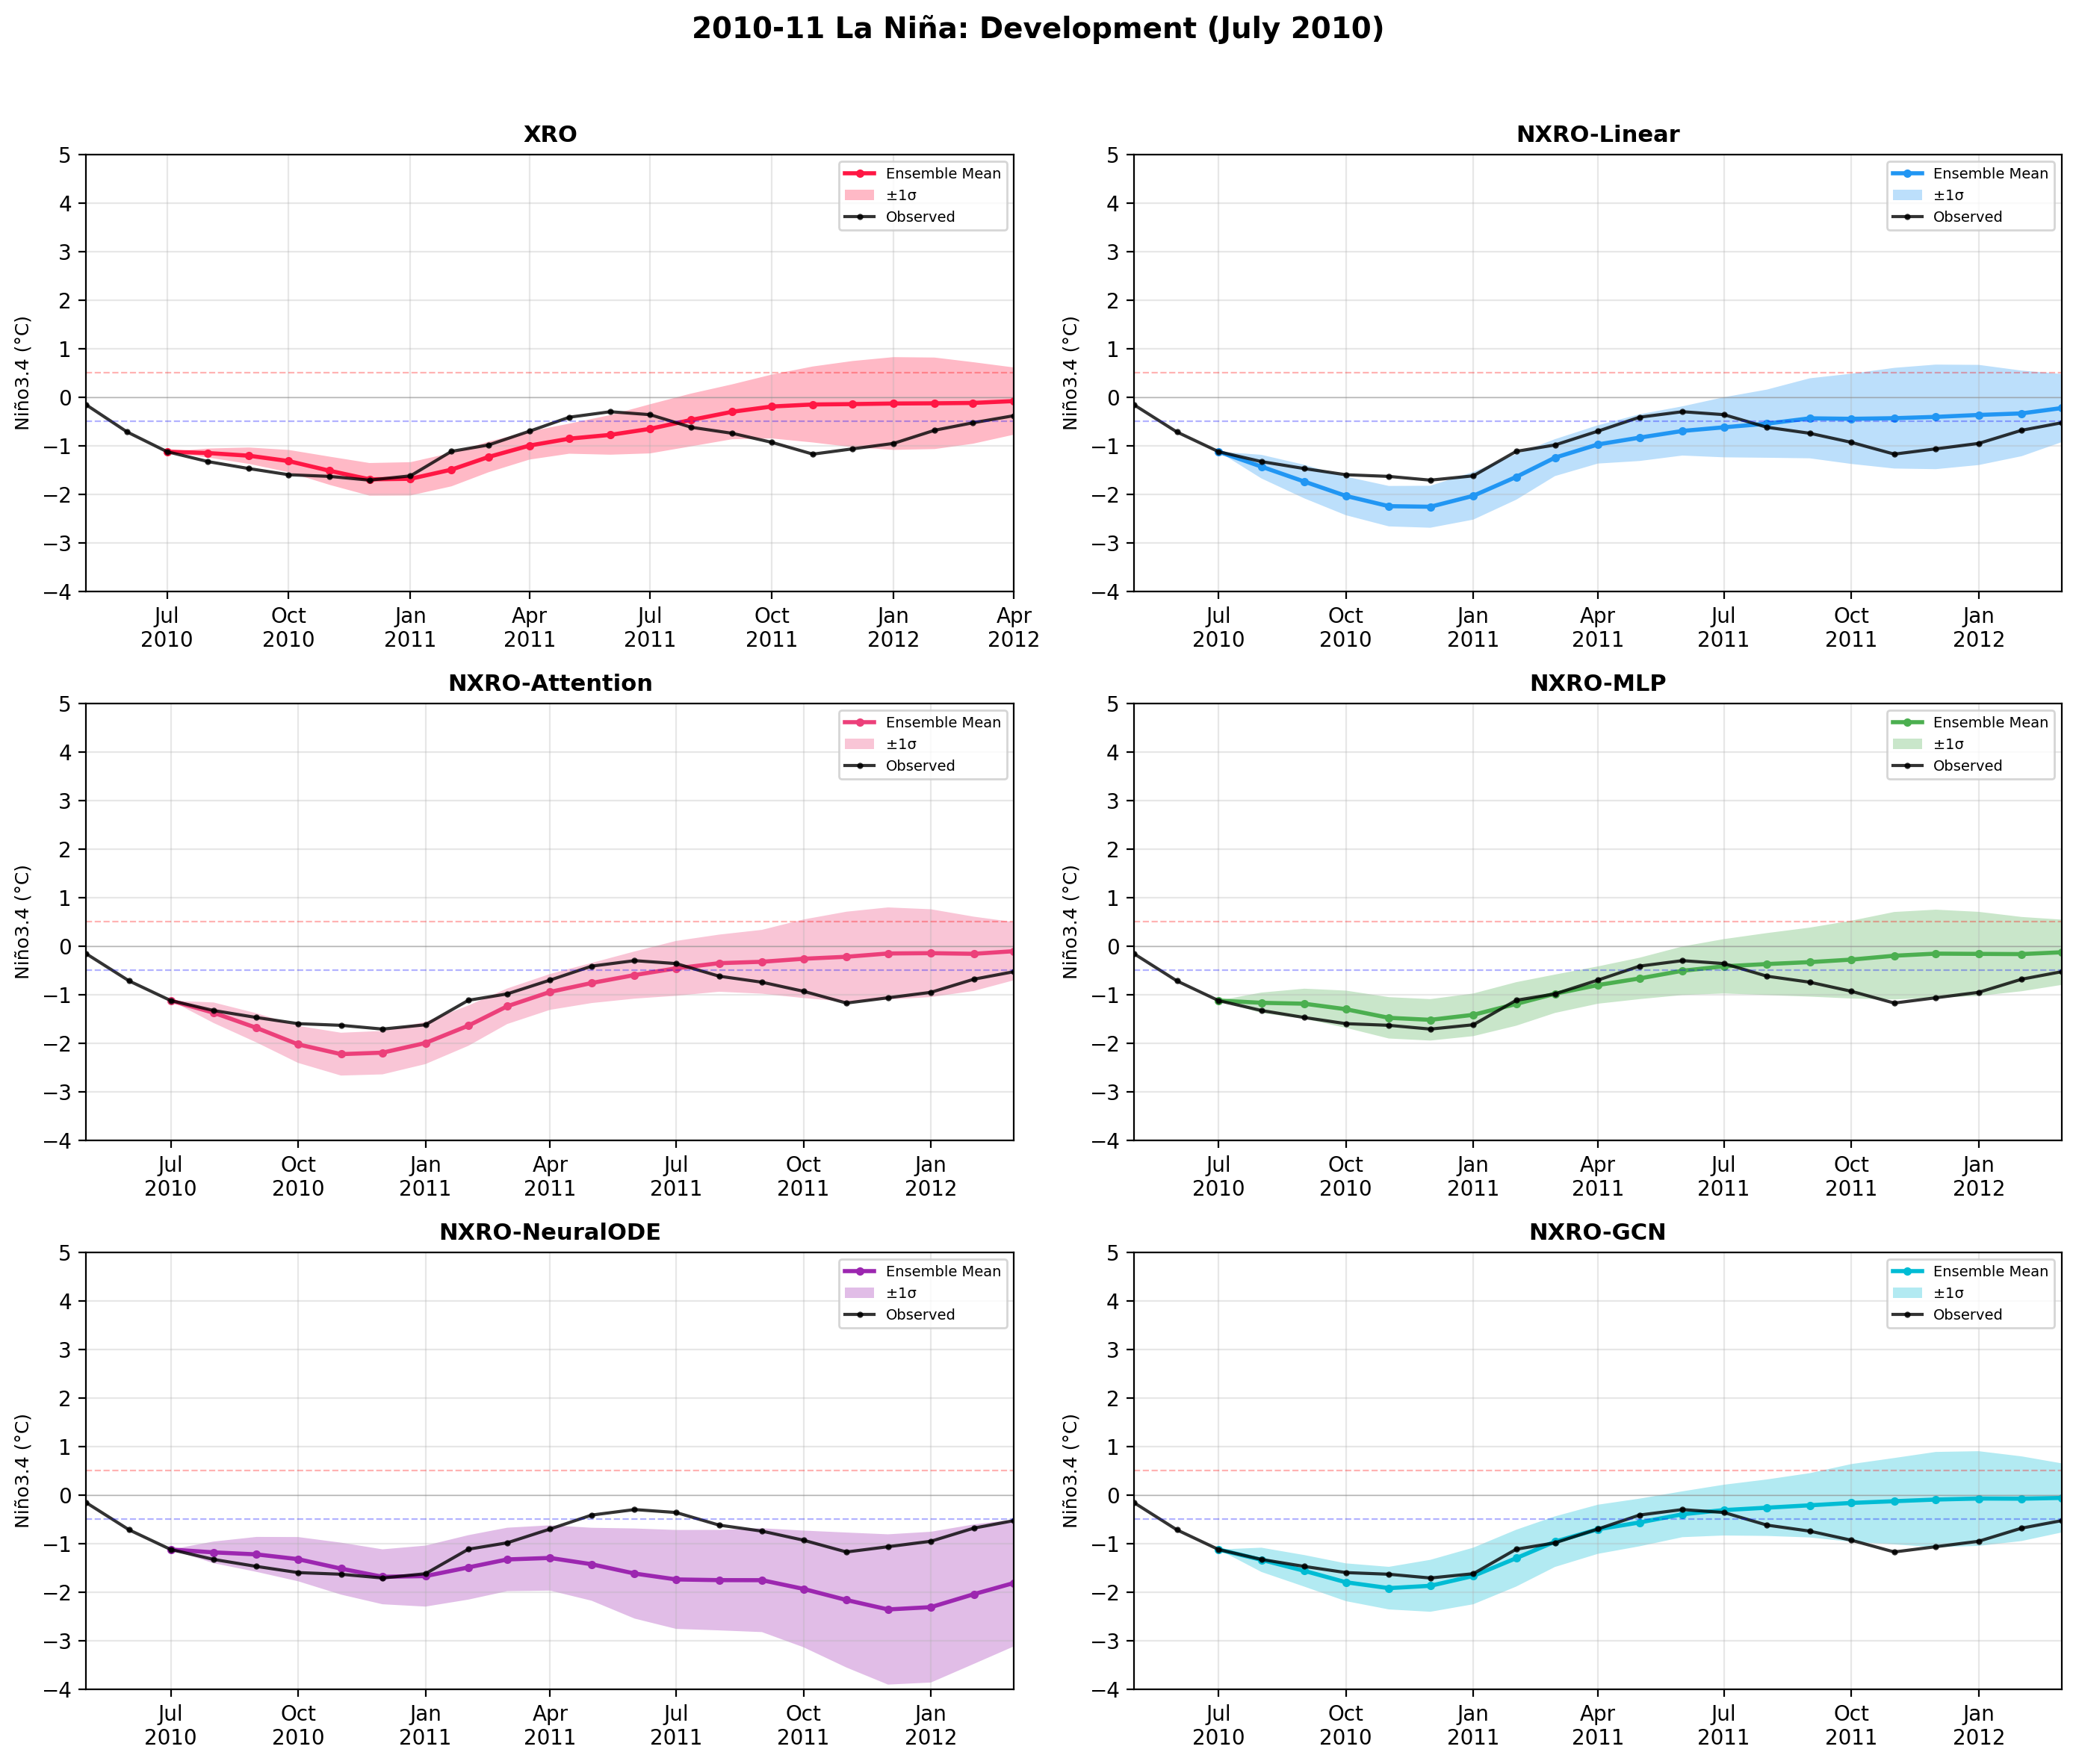
\includegraphics[width=\columnwidth]{figures/lanina_2010_dev.png}
  \caption{Stochastic forecast for 2010 La Ni\~na development. Ensemble forecast comparison.}
  \label{fig:2010_lanina}
\end{figure}
